% !TeX spellcheck = en_US
\documentclass[10pt,journal,compsoc]{IEEEtran}
%
% If IEEEtran.cls has not been installed into the LaTeX system files,
% manually specify the path to it like:
% \documentclass[10pt,journal,compsoc]{../sty/IEEEtran}





% Some very useful LaTeX packages include:
% (uncomment the ones you want to load)


% *** MISC UTILITY PACKAGES ***
%
%\usepackage{ifpdf}
% Heiko Oberdiek's ifpdf.sty is very useful if you need conditional
% compilation based on whether the output is pdf or dvi.
% usage:
% \ifpdf
%   % pdf code
% \else
%   % dvi code
% \fi
% The latest version of ifpdf.sty can be obtained from:
% http://www.ctan.org/pkg/ifpdf
% Also, note that IEEEtran.cls V1.7 and later provides a builtin
% \ifCLASSINFOpdf conditional that works the same way.
% When switching from latex to pdflatex and vice-versa, the compiler may
% have to be run twice to clear warning/error messages.






% *** CITATION PACKAGES ***
%
\ifCLASSOPTIONcompsoc
  % IEEE Computer Society needs nocompress option
  % requires cite.sty v4.0 or later (November 2003)
  \usepackage[nocompress]{cite}
\else
  % normal IEEE
  \usepackage{cite}
\fi
% cite.sty was written by Donald Arseneau
% V1.6 and later of IEEEtran pre-defines the format of the cite.sty package
% \cite{} output to follow that of the IEEE. Loading the cite package will
% result in citation numbers being automatically sorted and properly
% "compressed/ranged". e.g., [1], [9], [2], [7], [5], [6] without using
% cite.sty will become [1], [2], [5]--[7], [9] using cite.sty. cite.sty's
% \cite will automatically add leading space, if needed. Use cite.sty's
% noadjust option (cite.sty V3.8 and later) if you want to turn this off
% such as if a citation ever needs to be enclosed in parenthesis.
% cite.sty is already installed on most LaTeX systems. Be sure and use
% version 5.0 (2009-03-20) and later if using hyperref.sty.
% The latest version can be obtained at:
% http://www.ctan.org/pkg/cite
% The documentation is contained in the cite.sty file itself.
%
% Note that some packages require special options to format as the Computer
% Society requires. In particular, Computer Society  papers do not use
% compressed citation ranges as is done in typical IEEE papers
% (e.g., [1]-[4]). Instead, they list every citation separately in order
% (e.g., [1], [2], [3], [4]). To get the latter we need to load the cite
% package with the nocompress option which is supported by cite.sty v4.0
% and later. Note also the use of a CLASSOPTION conditional provided by
% IEEEtran.cls V1.7 and later.





% *** GRAPHICS RELATED PACKAGES ***
%
\ifCLASSINFOpdf
  \usepackage[pdftex]{graphicx}
  % declare the path(s) where your graphic files are
  \graphicspath{{../pdf/}{../jpeg/}}
  % and their extensions so you won't have to specify these with
  % every instance of \includegraphics
  \DeclareGraphicsExtensions{.pdf,.jpeg,.png}
\else
  % or other class option (dvipsone, dvipdf, if not using dvips). graphicx
  % will default to the driver specified in the system graphics.cfg if no
  % driver is specified.
  \usepackage[dvips]{graphicx}
  % declare the path(s) where your graphic files are
  \graphicspath{{../eps/}}
  % and their extensions so you won't have to specify these with
  % every instance of \includegraphics
  \DeclareGraphicsExtensions{.eps}
\fi
% graphicx was written by David Carlisle and Sebastian Rahtz. It is
% required if you want graphics, photos, etc. graphicx.sty is already
% installed on most LaTeX systems. The latest version and documentation
% can be obtained at: 
% http://www.ctan.org/pkg/graphicx
% Another good source of documentation is "Using Imported Graphics in
% LaTeX2e" by Keith Reckdahl which can be found at:
% http://www.ctan.org/pkg/epslatex
%
% latex, and pdflatex in dvi mode, support graphics in encapsulated
% postscript (.eps) format. pdflatex in pdf mode supports graphics
% in .pdf, .jpeg, .png and .mps (metapost) formats. Users should ensure
% that all non-photo figures use a vector format (.eps, .pdf, .mps) and
% not a bitmapped formats (.jpeg, .png). The IEEE frowns on bitmapped formats
% which can result in "jaggedy"/blurry rendering of lines and letters as
% well as large increases in file sizes.
%
% You can find documentation about the pdfTeX application at:
% http://www.tug.org/applications/pdftex






% *** MATH PACKAGES ***
%
\usepackage{amsmath}
% A popular package from the American Mathematical Society that provides
% many useful and powerful commands for dealing with mathematics.
%
% Note that the amsmath package sets \interdisplaylinepenalty to 10000
% thus preventing page breaks from occurring within multiline equations. Use:
%\interdisplaylinepenalty=2500
% after loading amsmath to restore such page breaks as IEEEtran.cls normally
% does. amsmath.sty is already installed on most LaTeX systems. The latest
% version and documentation can be obtained at:
% http://www.ctan.org/pkg/amsmath





% *** SPECIALIZED LIST PACKAGES ***
%
%\usepackage{algorithmic}
% algorithmic.sty was written by Peter Williams and Rogerio Brito.
% This package provides an algorithmic environment fo describing algorithms.
% You can use the algorithmic environment in-text or within a figure
% environment to provide for a floating algorithm. Do NOT use the algorithm
% floating environment provided by algorithm.sty (by the same authors) or
% algorithm2e.sty (by Christophe Fiorio) as the IEEE does not use dedicated
% algorithm float types and packages that provide these will not provide
% correct IEEE style captions. The latest version and documentation of
% algorithmic.sty can be obtained at:
% http://www.ctan.org/pkg/algorithms
% Also of interest may be the (relatively newer and more customizable)
% algorithmicx.sty package by Szasz Janos:
% http://www.ctan.org/pkg/algorithmicx




% *** ALIGNMENT PACKAGES ***
%
\usepackage{array}
% Frank Mittelbach's and David Carlisle's array.sty patches and improves
% the standard LaTeX2e array and tabular environments to provide better
% appearance and additional user controls. As the default LaTeX2e table
% generation code is lacking to the point of almost being broken with
% respect to the quality of the end results, all users are strongly
% advised to use an enhanced (at the very least that provided by array.sty)
% set of table tools. array.sty is already installed on most systems. The
% latest version and documentation can be obtained at:
% http://www.ctan.org/pkg/array


% IEEEtran contains the IEEEeqnarray family of commands that can be used to
% generate multiline equations as well as matrices, tables, etc., of high
% quality.




% *** SUBFIGURE PACKAGES ***
%\ifCLASSOPTIONcompsoc
%  \usepackage[caption=false,font=footnotesize,labelfont=sf,textfont=sf]{subfig}
%\else
%  \usepackage[caption=false,font=footnotesize]{subfig}
%\fi
% subfig.sty, written by Steven Douglas Cochran, is the modern replacement
% for subfigure.sty, the latter of which is no longer maintained and is
% incompatible with some LaTeX packages including fixltx2e. However,
% subfig.sty requires and automatically loads Axel Sommerfeldt's caption.sty
% which will override IEEEtran.cls' handling of captions and this will result
% in non-IEEE style figure/table captions. To prevent this problem, be sure
% and invoke subfig.sty's "caption=false" package option (available since
% subfig.sty version 1.3, 2005/06/28) as this is will preserve IEEEtran.cls
% handling of captions.
% Note that the Computer Society format requires a sans serif font rather
% than the serif font used in traditional IEEE formatting and thus the need
% to invoke different subfig.sty package options depending on whether
% compsoc mode has been enabled.
%
% The latest version and documentation of subfig.sty can be obtained at:
% http://www.ctan.org/pkg/subfig




% *** FLOAT PACKAGES ***
%
%\usepackage{fixltx2e}
% fixltx2e, the successor to the earlier fix2col.sty, was written by
% Frank Mittelbach and David Carlisle. This package corrects a few problems
% in the LaTeX2e kernel, the most notable of which is that in current
% LaTeX2e releases, the ordering of single and double column floats is not
% guaranteed to be preserved. Thus, an unpatched LaTeX2e can allow a
% single column figure to be placed prior to an earlier double column
% figure.
% Be aware that LaTeX2e kernels dated 2015 and later have fixltx2e.sty's
% corrections already built into the system in which case a warning will
% be issued if an attempt is made to load fixltx2e.sty as it is no longer
% needed.
% The latest version and documentation can be found at:
% http://www.ctan.org/pkg/fixltx2e


%\usepackage{stfloats}
% stfloats.sty was written by Sigitas Tolusis. This package gives LaTeX2e
% the ability to do double column floats at the bottom of the page as well
% as the top. (e.g., "\begin{figure*}[!b]" is not normally possible in
% LaTeX2e). It also provides a command:
%\fnbelowfloat
% to enable the placement of footnotes below bottom floats (the standard
% LaTeX2e kernel puts them above bottom floats). This is an invasive package
% which rewrites many portions of the LaTeX2e float routines. It may not work
% with other packages that modify the LaTeX2e float routines. The latest
% version and documentation can be obtained at:
% http://www.ctan.org/pkg/stfloats
% Do not use the stfloats baselinefloat ability as the IEEE does not allow
% \baselineskip to stretch. Authors submitting work to the IEEE should note
% that the IEEE rarely uses double column equations and that authors should try
% to avoid such use. Do not be tempted to use the cuted.sty or midfloat.sty
% packages (also by Sigitas Tolusis) as the IEEE does not format its papers in
% such ways.
% Do not attempt to use stfloats with fixltx2e as they are incompatible.
% Instead, use Morten Hogholm'a dblfloatfix which combines the features
% of both fixltx2e and stfloats:
%
% \usepackage{dblfloatfix}
% The latest version can be found at:
% http://www.ctan.org/pkg/dblfloatfix




\ifCLASSOPTIONcaptionsoff
  \usepackage[nomarkers]{endfloat}
 \let\MYoriglatexcaption\caption
 \renewcommand{\caption}[2][\relax]{\MYoriglatexcaption[#2]{#2}}
\fi
% endfloat.sty was written by James Darrell McCauley, Jeff Goldberg and 
% Axel Sommerfeldt. This package may be useful when used in conjunction with 
% IEEEtran.cls'  captionsoff option. Some IEEE journals/societies require that
% submissions have lists of figures/tables at the end of the paper and that
% figures/tables without any captions are placed on a page by themselves at
% the end of the document. If needed, the draftcls IEEEtran class option or
% \CLASSINPUTbaselinestretch interface can be used to increase the line
% spacing as well. Be sure and use the nomarkers option of endfloat to
% prevent endfloat from "marking" where the figures would have been placed
% in the text. The two hack lines of code above are a slight modification of
% that suggested by in the endfloat docs (section 8.4.1) to ensure that
% the full captions always appear in the list of figures/tables - even if
% the user used the short optional argument of \caption[]{}.
% IEEE papers do not typically make use of \caption[]'s optional argument,
% so this should not be an issue. A similar trick can be used to disable
% captions of packages such as subfig.sty that lack options to turn off
% the subcaptions:
% For subfig.sty:
% \let\MYorigsubfloat\subfloat
% \renewcommand{\subfloat}[2][\relax]{\MYorigsubfloat[]{#2}}
% However, the above trick will not work if both optional arguments of
% the \subfloat command are used. Furthermore, there needs to be a
% description of each subfigure *somewhere* and endfloat does not add
% subfigure captions to its list of figures. Thus, the best approach is to
% avoid the use of subfigure captions (many IEEE journals avoid them anyway)
% and instead reference/explain all the subfigures within the main caption.
% The latest version of endfloat.sty and its documentation can obtained at:
% http://www.ctan.org/pkg/endfloat
%
% The IEEEtran \ifCLASSOPTIONcaptionsoff conditional can also be used
% later in the document, say, to conditionally put the References on a 
% page by themselves.




% *** PDF, URL AND HYPERLINK PACKAGES ***
%
\usepackage{url}
% url.sty was written by Donald Arseneau. It provides better support for
% handling and breaking URLs. url.sty is already installed on most LaTeX
% systems. The latest version and documentation can be obtained at:
% http://www.ctan.org/pkg/url
% Basically, \url{my_url_here}.





% *** Do not adjust lengths that control margins, column widths, etc. ***
% *** Do not use packages that alter fonts (such as pslatex).         ***
% There should be no need to do such things with IEEEtran.cls V1.6 and later.
% (Unless specifically asked to do so by the journal or conference you plan
% to submit to, of course. )


% correct bad hyphenation here
\hyphenation{op-tical net-works semi-conduc-tor}

%%%%%%%%%%%%%%%%%%%%%%%%%%%%%%%%%%%%%%%%%%%%%%%%%%%%%%%%%%%%
%% Custom Packages not from the template
%%%%%%%%%%%%%%%%%%%%%%%%%%%%%%%%%%%%%%%%%%%%%%%%%%%%%%%%%%%%
\usepackage{nth}
\usepackage{hyperref}

\begin{document}
%
% paper title
% Titles are generally capitalized except for words such as a, an, and, as,
% at, but, by, for, in, nor, of, on, or, the, to and up, which are usually
% not capitalized unless they are the first or last word of the title.
% Linebreaks \\ can be used within to get better formatting as desired.
% Do not put math or special symbols in the title.
\title{Unobservable Messaging with MessageVortex}
%
%
% author names and IEEE memberships
% note positions of commas and nonbreaking spaces ( ~ ) LaTeX will not break
% a structure at a ~ so this keeps an author's name from being broken across
% two lines.
% use \thanks{} to gain access to the first footnote area
% a separate \thanks must be used for each paragraph as LaTeX2e's \thanks
% was not built to handle multiple paragraphs
%
%
%\IEEEcompsocitemizethanks is a special \thanks that produces the bulleted
% lists the Computer Society journals use for "first footnote" author
% affiliations. Use \IEEEcompsocthanksitem which works much like \item
% for each affiliation group. When not in compsoc mode,
% \IEEEcompsocitemizethanks becomes like \thanks and
% \IEEEcompsocthanksitem becomes a line break with idention. This
% facilitates dual compilation, although admittedly the differences in the
% desired content of \author between the different types of papers makes a
% one-size-fits-all approach a daunting prospect. For instance, compsoc 
% journal papers have the author affiliations above the "Manuscript
% received ..."  text while in non-compsoc journals this is reversed. Sigh.

\author{Martin~Gwerder%,~\IEEEmembership{Member,~IEEE,}
        %John~Doe,~\IEEEmembership{Fellow,~OSA,}

\IEEEcompsocitemizethanks{\IEEEcompsocthanksitem M. Gwerder was with the Institute of Mobile and Distributed Systems
of the University of Applied Sciences of Northwestern Switzerland.\protect\\
% note need leading \protect in front of \\ to get a newline within \thanks as
% \\ is fragile and will error, could use \hfil\break instead.
E-mail: see http://www.messagevortex.net
%\IEEEcompsocthanksitem J. Doe and J. Doe are with Anonymous University.
}% <-this % stops an unwanted space
\thanks{Manuscript received June 1, 2019; revised July 20, 2019.}
        }% <-this % stops a space

% note the % following the last \IEEEmembership and also \thanks - 
% these prevent an unwanted space from occurring between the last author name
% and the end of the author line. i.e., if you had this:
% 
% \author{....lastname \thanks{...} \thanks{...} }
%                     ^------------^------------^----Do not want these spaces!
%
% a space would be appended to the last name and could cause every name on that
% line to be shifted left slightly. This is one of those "LaTeX things". For
% instance, "\textbf{A} \textbf{B}" will typeset as "A B" not "AB". To get
% "AB" then you have to do: "\textbf{A}\textbf{B}"
% \thanks is no different in this regard, so shield the last } of each \thanks
% that ends a line with a % and do not let a space in before the next \thanks.
% Spaces after \IEEEmembership other than the last one are OK (and needed) as
% you are supposed to have spaces between the names. For what it is worth,
% this is a minor point as most people would not even notice if the said evil
% space somehow managed to creep in.



% The paper headers
\markboth{Journal Privacy \& Anonymity,~Vol.~XXXX, No.~XXXX, September~2019}%
{Gwerder \MakeLowercase{\textit{et al.}}: Unobservable Messaging wit Messagevortex}
% The only time the second header will appear is for the odd numbered pages
% after the title page when using the twoside option.
% 
% *** Note that you probably will NOT want to include the author's ***
% *** name in the headers of peer review papers.                   ***
% You can use \ifCLASSOPTIONpeerreview for conditional compilation here if
% you desire.



% The publisher's ID mark at the bottom of the page is less important with
% Computer Society journal papers as those publications place the marks
% outside of the main text columns and, therefore, unlike regular IEEE
% journals, the available text space is not reduced by their presence.
% If you want to put a publisher's ID mark on the page you can do it like
% this:
%\IEEEpubid{0000--0000/00\$00.00~\copyright~2015 IEEE}
% or like this to get the Computer Society new two part style.
%\IEEEpubid{\makebox[\columnwidth]{\hfill 0000--0000/00/\$00.00~\copyright~2015 IEEE}%
%\hspace{\columnsep}\makebox[\columnwidth]{Published by the IEEE Computer Society\hfill}}
% Remember, if you use this you must call \IEEEpubidadjcol in the second
% column for its text to clear the IEEEpubid mark (Computer Society jorunal
% papers don't need this extra clearance.)



% use for special paper notices
%\IEEEspecialpapernotice{(Invited Paper)}



% for Computer Society papers, we must declare the abstract and index terms
% PRIOR to the title within the \IEEEtitleabstractindextext IEEEtran
% command as these need to go into the title area created by \maketitle.
% As a general rule, do not put math, special symbols or citations
% in the abstract or keywords.
\IEEEtitleabstractindextext{%
\begin{abstract}
In this paper, we introduce an unobservable message anonymization protocol, named MessageVortex. It bases on the zero trust principle and a distributed peer-to-peer like architecture and avoids central aspects such as fixed infrastructures within a global network. 

It scores over existing work by blending its traffic into suitable existing transport protocols, thus making it next to impossible to block it without significantly affecting regular users of the transport medium. No additional protocol-specific infrastructure is required in public networks and allows a sender to control all aspects of a message such as the degree of anonymity, timing, and redundancy of the message transport without disclosing any of these details to the routing or transporting nodes. Part of this work is an RFC document attached in Appendix \ref{app:rfcMessageVortexMain} describing the protocol. It contains all the necessary information to build protocol nodes. The RFC draft is available through the official RFC channels. Additionally, the RFC document, additional documents, and a reference are available under \url{https://messagevortex.net/}.
\end{abstract}

% Note that keywords are not normally used for peerreview papers.
\begin{IEEEkeywords}
Computer Society, IEEE, IEEEtran, journal, \LaTeX, paper, template.
\end{IEEEkeywords}}


% make the title area
\maketitle


% To allow for easy dual compilation without having to reenter the
% abstract/keywords data, the \IEEEtitleabstractindextext text will
% not be used in maketitle, but will appear (i.e., to be "transported")
% here as \IEEEdisplaynontitleabstractindextext when the compsoc 
% or transmag modes are not selected <OR> if conference mode is selected 
% - because all conference papers position the abstract like regular
% papers do.
\IEEEdisplaynontitleabstractindextext
% \IEEEdisplaynontitleabstractindextext has no effect when using
% compsoc or transmag under a non-conference mode.



% For peer review papers, you can put extra information on the cover
% page as needed:
% \ifCLASSOPTIONpeerreview
% \begin{center} \bfseries EDICS Category: 3-BBND \end{center}
% \fi
%
% For peerreview papers, this IEEEtran command inserts a page break and
% creates the second title. It will be ignored for other modes.
\IEEEpeerreviewmaketitle



\IEEEraisesectionheading{\section{Introduction}\label{sec:introduction}}
% Computer Society journal (but not conference!) papers do something unusual
% with the very first section heading (almost always called "Introduction").
% They place it ABOVE the main text! IEEEtran.cls does not automatically do
% this for you, but you can achieve this effect with the provided
% \IEEEraisesectionheading{} command. Note the need to keep any \label that
% is to refer to the section immediately after \section in the above as
% \IEEEraisesectionheading puts \section within a raised box.




% The very first letter is a 2 line initial drop letter followed
% by the rest of the first word in caps (small caps for compsoc).
% 
% form to use if the first word consists of a single letter:
% \IEEEPARstart{A}{demo} file is ....
% 
% form to use if you need the single drop letter followed by
% normal text (unknown if ever used by the IEEE):
% \IEEEPARstart{A}{}demo file is ....
% 
% Some journals put the first two words in caps:
% \IEEEPARstart{T}{his demo} file is ....
% 
% Here we have the typical use of a "T" for an initial drop letter
% and "HIS" in caps to complete the first word.
\IEEEPARstart{A}{lmon Brown Strowger} was the owner of a funeral parlor in St. Petersburg. He filed a patent on March \nth{10}, 1891 for an ``Automatic Telephone Exchange'' \cite{pulseDialingPatent}. This patent built the base for modern automated telephone systems. According to several sources, he was annoyed by the fact that the local telephone operator was married to another undertaker. She diverted potential customers of Mr. Strowger to her husband instead, which caused Almon B. Strowger to lose business. In 1922, this telephone dialing system which is nowadays called pulse dialing became the standard dialing technology for more than 70 years until tone dialing replaced it.

This dialing technology enabled automatic messaging for voice and text messages (e.g. telex) up until today and is the foundation for current routed networks. These networks build the base for our communication-based Society these days and allow us to connect quickly with any person or company of our wish. We use these networks today as communication meaning for all purposes and most of the people spend minimal thoughts on the possible consequences arising if someone puts hands on this communication. 

Collected data may be used to judge on our intentions and thus is not only confidential if we have something to hide. This problem has dramatically increased in the last years as big companies and countries started to collect all kinds of data and created the means to process them. It allows, supposedly, to judge peoples not only on what they are doing but as well, on what they did and what they might do. Numerous events in the present and past show that multiple actors, some of which are state-sponsored, collected data on a broad base within the internet. Whether this is a problem or not may be disputable. Undisputed is that such data requires careful handling and accusations should then base on solid facts. Unacceptable seems the use of ``guesses'' or ``extrapolations'' in most of the cases.

To show that this may happen even under complete democratic control we might refer to events such as the ``secret files scandal'' (or  ``Fichenskandal'') in Switzerland. In the years from 1900 to 1990 Swiss government collected 900’000 files in a secret archive (covering roughly 10\% of the natural and juristic entities within Switzerland at that time). More about the Fichenskandal is well documented in the Swiss Federal Archives (https://www.bar.admin.ch).

Whistleblower Edward Snowden leaked a vast amount of documents suggesting that such attacks on privacy are commonly done a on a global scale. The documents were leaked in 2009 and a significant number of journalists from multiple countries screened these documents (\href{http://www.nrc.nl/nieuws/2013/11/23/nederland-sinds-1946-doelwit-van-nsa}{NRC}). According to these documents, NSA infiltrated more than 50k computers with malware to collect classified or personal information. They furthermore infiltrated Telecom-Operators (mainly executed by British GCHQ) such as Belgacom to collect data and targeted high member of governments even in associated states (such as the mobile phone number of Germany's president and high ranking members of economy and finance).

This list of events shows that big players are collecting and storing vast amounts of data for analysis or possibly future use. The list of events shows also that the use of this data has in the past been at least partially questionable. As a part of possible counter measures this work analyses the possibility of using state-of-the-art technology to minimize the information footprint of a person on the Internet. 

We leave a vast information footprint in our daily communication. On a regular email we disclose everything in an ``postcard'' to any entity on its way. Even when encrypting a message perfectly with today's technology (S/MIME\cite{RFC2045} or PGP\cite{RFC2015}) it still leaves at least the originating and the receiving entity disclosed or we rely on the promises of a third party provider which offers a proprietary solution. Even in those cases we leak informations such as ``message subject'', ``frequency of exchanged messages'', ``size of messages'', or ``client beeing used''. A good anonymity protocol has therefore far more attributes to cover than the message itself. It includes beside the message itself, all metadata, and all the traffic flows. Furthermore, a protocol to anonymize messages should not rely on the trust of infrastructure other than the infrastructure under control of the sending or receiving entity. A trust in any third party might be misleading in terms of security.

Central infrastructure is bound to be of particular interest to anyone gathering data. It may furthermore allow manipulating the system or the data or the data flow. So, avoiding a central infrastructure is a good thing.

Leaving no information trail when sending information from one person to another is hard to achieve. Most messaging systems disclose at least the peer partners when sending messages. Metadata such as starting and endpoints, frequency, or message size are leaked in all common systems even when encrypting messages.

Allowing an entity to collect data may affect senders and recipients of any information. Collection of vast amounts of data allows a potent adversary to build a  profile of a person. Unlike in the past, the availability of this kind of information has been risen to a never known extend with the internet.

An entity in possession of such Profiles may use them for many purposes. These include service adoption, directed advertising or classification of citizens. The examples given above show that the effects of this data is not limited to the internet but reaches us effectively in the real world.

The main problem of this data is that it may be collected over a considerable amount of time and evaluated at any time. It even happened that standard practices of a time are differently judged upon in a later time. Persons may then be judged retrospectively upon these types of practice. This questionable type of judgment is visible in the tax avoidance discussion. 

People must be able to control their data footprint. Not providing these means does effectively allow any country or a bigger player to ban and control any number of persons within or outside the internet. 

In this work, a new protocol is designed to allow message transfer through existing communication channels. These messages are next to unobservable to any third party. This unobservability does not only cover the message itself but all metadata and flows associated with it. We called this protocol ``MessageVortex'' or in short just ``Vortex''. The protocol is designed in such a way so that it is capable of using a wide variety of transport protocols. It is even possible to switch protocols while the messages are in transfer. This behavior allows media breaches (at least on a protocol level) and makes analysis even harder.

The new protocol allows secure communication without the need for trusting the underlying transport media. Furthermore, the usage of the protocol itself is possible without altering the immediate behavior of the transport layer. That way it is possible to use the transport layers normal traffic to increase the noise in which information has to be searched. 

\subsection{About Unlinkability, Unobservability, Undetectability and Censorship resistance}
From an academic point of view achieving anonymity is relatively simple. All we need is a trusted party distributing the messages while making sure that no trace from the sender arrives at the recipient. Unlinkability as defined in \cite{anon_terminology} is much harder to achieve. It requires that a specified attacker is unable to link a sender and recipients of a message. Even if a system provides unlinkable message transfer, it is most probable prone to denial of service and thus partial or full censorship. By introducing a global observer or infiltrating parts of the system an attacker may gain insight int the messages transported by the system and thus leaking information.

So in order to be censorship resistant a protocol requires a number of very important and not so obvious properties. As outlined It should be undetectable from the outside. From within the system we need to provide 

MessageVortex is a protocol providing under ideal circumstances censorship resistance. It does this using a rigid design from bottom up to provide the required properties. While being a protocol on its own, it uses many common protocols. Partly to provide user friendliness, but mostly to hide within the common network flows. As such a protocol requires to be undetectable on the network. A protocol all alone may not be undetectable as each protocol sends data over a network. This data is detectable. In order to be undetectable a censorship resistant protocol requires to be embedded undetectably in legit message flows. This is usually done either by side channel transmissions or by employing steganography. Our Protocol may use both but will use typically the later. 

\section{The MessageVortex Protocol}
The theory in this document is heavily based on symmetric encryption, asymmetric encryption and hashing. In order to use a uniformed notation I use $E^{K_a}(M)$ (where $a$ is an index to distinguish multiple keys) resulting in $\mathbf{M^{K_a}}$ as the encrypted message. If we are reflecting a tuple of information we write it in boldface. to express the tuples content we use angular brackets $\mathbf{L\langle normalAddress,vortexAddress\rangle }$. If we want Messages encrypted with multiple keys do list the used keys as a comma separated list in superscript $E^{K_b}\left(E^{K_a}\left(M\right)\right)=M^{{K_{a}},{K_b}}$.

For a symmetric encryption of a message $\mathbf{M}$ with a key $K_a$ resulting in $\mathbf{M^{K_a}}$ where $a$ is an index to distinguish different keys. Decryption uses therefore $D^{K_a}(\mathbf{M^{K_a}})=\mathbf{M}$.

As notation for asymetric encryption we use $E^{K^{1}_a}(\mathbf{M})$ where as $K^{-1}_a$ is the private key and $K^{1}_a$ is the public key of a key pair $K^p_a$. The asymmetric decryption is noted as $D^{K^{-1}_a}(\mathbf{M})$.

For hashing we do use $H(\mathbf{M})$ if unsalted and $H^{S_a}$ if using a salted hash with salt $S_a$. The generated hash is shown as $H_M$ if unsalted and $H^{S_a}_M$ if salted.

If we want to express what details contained in a tuple we use the the notation $\mathbf{M\langle t,MURB,serial\rangle }$ respectively if encrypted $\mathbf{M^{K_{a}}\langle t,MURB,serial\rangle}$.

\begin{align*}
\text{asymetric:}         & E^{K^{-1}_a}\left(\mathbf{M}\right)                        	&& =\mathbf{M}^{K^{-1}_a}\\
& D^{K^{1}_a}\left(E^{K^{-1}_a}\left(\mathbf{M}\right)\right)	&& =\mathbf{M}\\
& D^{K^{-1}_a}\left(E^{K^{1}_a}\left(\mathbf{M}\right)\right)	&& =\mathbf{M}\\
\text{symetric:}          & E^{K_a}\left(\mathbf{M}\right)                             	&& =\mathbf{M}^{K_a}\\
& D^{K_a}\left(E^{K_a}\left(\mathbf{M}\right)\right)          && =\mathbf{M}\\
\text{hashing (unsalted):}& H\left(\mathbf{M}\right)                                   	&& =\mathbf{H}_M\\
\text{hashing (salted):}  & H^{S_a}\left(\mathbf{M}\right)                             	&& =\mathbf{H}^{S_a}_M
\end{align*}

In general Subscripts denote selectors to differentiate values of the same type and superscript denote relevant parameters to operations expressed. The subscripted and superscripted information may be omitted where not needed.

We refer to the components of a Vortex Message as follows:
\begin{align*}
\text{Prefix component:}         & \mathbf{PREFIX}             	&=D^{K^{1}_a}\left(\mathbf{P}^{K^{-1}_a}\right) &=D\left(\mathbf{P}\right)\\
\text{Header component:}         & \mathbf{HEAD}             	&=D^{K^{1}_a}\left(\mathbf{H}^{K^{-1}_a}\right) &=D\left(\mathbf{H}\right)\\
\text{Route component:}         & \mathbf{ROUTE}             	&=D^{K^{1}_a}\left(\mathbf{R}^{K^{-1}_a}\right) &=D\left(\mathbf{R}\right)\\
\end{align*}

In general a decrypted Block is written as capitalized multi character boldface. An encrypted Block is written as capitalized single character boldface.

\subsection{General Design}
In this section, we introduce a new consistent, transport independent model for representing the different protocols used by MessageVortex.

\begin{figure}[ht!]
	\centering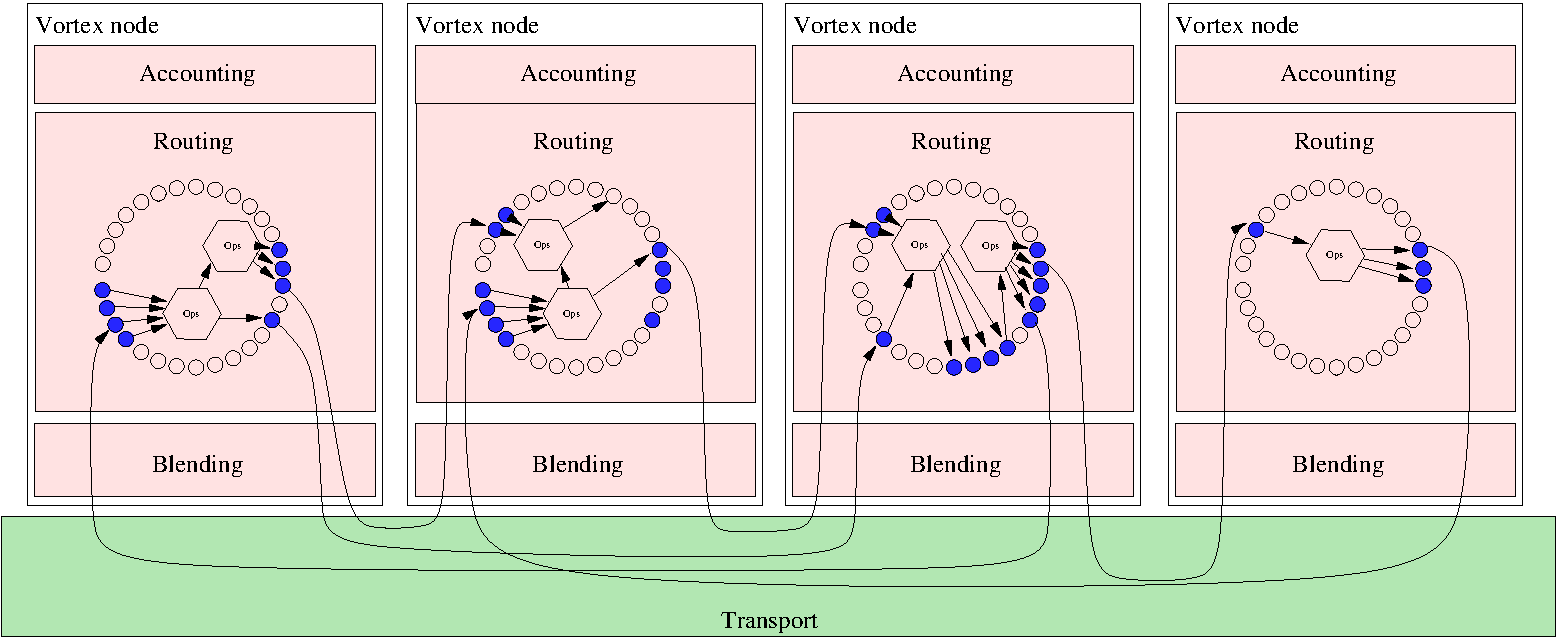
\includegraphics[width=\columnwidth]{../../inc/roughProtocolDesign.pdf}
	\caption{A rough protocol outline of the MessageVortex protocol}\label{fig:protocolOutline}
\end{figure}

We divide our protocol into four different layers, whereas only three are specific to the MessageVortex protocol. The lowest layer is the transport layer. As expressed earlier, dedicated protocols are easy to censor. Therefore we build our protocol on top of other suitable transport protocols. 

The other Three layers are vortex specific and do not require any infrastructure on the internet. We elaborate further on these layers in the next section.

For our first tests, we used a custom transport layer allowing us to monitor all traffic quickly, and build structures in a very flexible way. This transport layer works locally with a minimum amount of work for setup and deployment. It furthermore works across multiple hosts in a broadcast domain. The API may be used to support almost any kind of transport layer. After that, we focused on the protocols identified suitable as transport protocols:
\begin{itemize}
	\item SMTP
	\item XMPP
\end{itemize}
For the prototype, we have implemented an SMTP transport agent and the respective blending layer.

The blending layer is taking care of multiple problems:
\begin{itemize}
	\item It is translating the message block into a suitable format for transport\\
	This translation includes jobs such as embedding a block as encoded text, as a binary attachment or hide it within a message using steganography.
	\item Extract incoming blocks\\
	Identify incoming messages containing a possible block and extract it from the message.
	\item Do housekeeping on the storage layer of the transport protocol\\
	Access protocols POP and IMAP require that messages are deleted from time to time in order to stay below the sizing quotas of an account.      
\end{itemize}

We define the blending layer to work as follows when receiving messages:
\begin{enumerate}
	\item Log arrival time (in UTC) on the transport layer.
	\item Extract possible blocks.
	\item Apply decryption on a suspected header block.
	\item Identify header block as valid by querying the accounting.
	\item Extract and decrypt subsequent blocks.
	\item Pass extracted blocks and information to the routing layer.
\end{enumerate}

We define the blending layer to work as follows for sending messages:

\begin{enumerate}
	\item Assemble message as passed on by the routing layer.
	\item Using the blending method specified in the routing block build an empty message. 
	\item Create a message decoy content.
	\item Send the message to the appropriate recipient using the transport layer protocol.
\end{enumerate}

The routing layer receives the message blocks in a decrypted and authorized form from the blending layer and processes them as follows:

\begin{itemize}
	\item Build structure representing the block building and the appropriate block IDs.
	\item Schedule all Routing blocks for processing in an priority queue.
	\item Authorise all routing blocks ready for processing with the calculated block sizes.
	\item Process blocks.
	\item Send prepared building blocks to the Blending layer.
\end{itemize}

\subsubsection{Identities and Keys}
Several keys are being used during the life of a message. In the following section, we emphasize on the type, the usage, and their specialties.

\subsubsection{Peer key}
The peer key is a message specific symmetrical key known to two adjacent routing nodes. It is generated by the sending routing node and encrypted with the public key of the receiving nodes identity key.

\subsubsection{Header Key}
The header key is a symmetric key protecting the routing and ephemeral identity information of the message. It is prepended to the header section and protected by the identity key of the processing node.

The Identity key is a static, asymmetric keypair existing on a per user base used to sign messages or encrypt symmetric keys. We refer here as a user any peer participating in the message stream. Every user participating in the Vortex network requires at least one key pair. Depending on the use-case (e.g., unlikable signatures or scalable security) a user may use multiple key pairs at the same time.

An ephemeral identity key identifies the sender to a processing host. The ephemeral identity key must be handled in such a way that it is not linkable. It is mainly used to process accounting information.

\subsection{Messages}
The outline in figure \ref{fig:messageOutline} is a simplified view of the message block of MessageVortex.

\begin{figure*}[ht]
	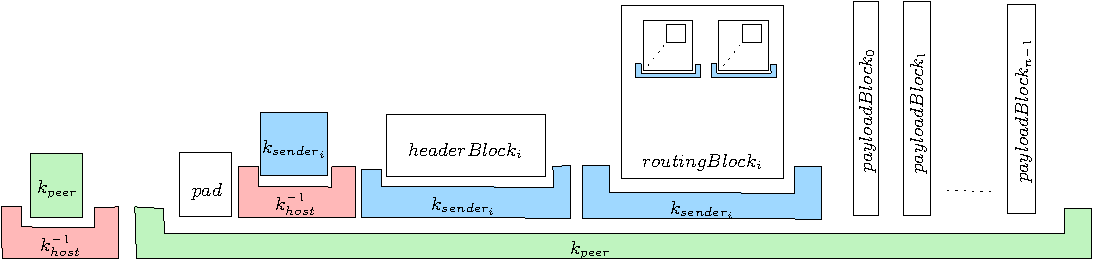
\includegraphics[width=\textwidth]{../../inc/blockLayoutSimplified}
	\caption{Simplified message outline}
	\label{fig:messageOutline}
\end{figure*}

A Vortex message is a message passed from one router to another this message may or may not contain any valuable information. Binary data represents the message content in the transfer protocol. Every router may decide for himself on the support of algorithms and embedding mechanisms.

The block structure of a Vortex message is as follows:
\begin{itemize}
	\item header
	\begin{itemize}
		\item Encrypted message key.\\
		Contains symmetrical key for decryption of follow up header information and payload blocks. All symmetric keys are encrypted with a receiving host's public key.
		\item Identity and ``proof of work'' information\\
		This information contains requests, proof-of-work sections, and a header key.
	\end{itemize}
	\item Encrypted payload blocks (encrypted with header key)
	\begin{itemize}
		\item Routing blocks (encrypted with message key)
		\begin{itemize}
			\item Next hop timing instructions
			\item Next hop routing blocks (encrypted)
			\item Next hop header
			\item Message build instructions.
			\item Next hop header key and spec.
			\item Next hop blending instructions.
		\end{itemize}
		\item Payload chunk blocks
	\end{itemize}
\end{itemize}

It is important to note that there are two symmetrical keys involved in encrypting and decrypting message headers. Having two keys is not a flaw in the protocol but necessary. 

The first key of a Vortex message is the message key. This key is only accessible with the private key of the node receiving the message. It allows decryption of the routing blocks and the header information. The sender of a message block is therefore not able to tell if a message contains one or more routing blocks. It is important to note that no other node should have access to this information. 

The second key is the header key located in the encrypted header. The RBB chooses the key. This key protects the inner structure of the Message. It makes it impossible for any node except the sending or the receiving peer node to detect the inner structure of the message. Without this key, any independent observer with knowledge about the blending capabilities of a receiving node may:
\begin{itemize}
	\item easier identify the block structure.\\ 
	This remains the case regardless of whether ASN.1 or length prefixed structures are used. If the structure of a vortex Message can be easily identified the messages may be logged or dropped.
	\item Identify the routing block size.\\
	The value of this information is only minimal as it only reflects the complexity of the remaining routing information indirectly.
	\item Identify the number of payload blocks and their respective sizes. \\
	This is valuable information when following traffic of a message.
\end{itemize}

\subsection{Transport and Blending Layer}
The tuple of Transport and Blending layer builds the main core functionality when it comes to the undetectability property. In order to avoid transport protocol misuse and unintentional exit nodes of the protocol the original RBL has no control over the transported content except for the hidden VortexMessage and how it is embedded. This loads the burden of sensible clear text payload generation to blending layer. It is relatively easy to generate a credible clear text message to pass an automated testing engine. This can be easily proven by looking at the effectivity of junk mail filters. These filters have tremendous problems continuosly adapting to the new types of unsolicited bulk emails (UBE).

Things do however drastically change if taking a human censor into account.

\subsubsection{Applied Steganography and the Dead Parrot}
A human censor is able to take very complex information into account when it comes to analyses of message content. He is able to not only analyze a message for its true content, but he may also see the message in the context of other messages. In \cite{oakland2013-parrot} is expressed that it is easy for a human to determine decoy traffic as the content is easily identifiable as generated content. While this is true, there is a possibility here to generate ``human-like'' data traffic to a certain extent. As an adversary may not assume that his messages are replied to, the problem does not boil down to a true Turing test. It remains on a ``passive observer Turing test'', enabling the potential nodes to choose their messages. 

For steganography we decided to go for F5\cite{f5}. It is a reasonably well-researched algorithm which attracted many researchers. The original F5 implementation had a detectable issue with artifacts\cite{F5broken} caused by the recompression of the image. This issue was caused only due to an issue in the reference implementation, and the researchers have provided a corrected reference implementation without the weakness. Like always the type of embedding may be specified and replaced upon request. 

\subsection{Routing and Accounting}
Each routing layer does the anonymization operations. These operations should make sure that no message may be identified unless destined for the current node. 

\subsection{The Core: Operations}
We differentiate three types of operations:
\begin{itemize}
	\item Splitting and merging of chunks
	\item Encryption and decryption of chunks
	\item Redundancy calculations carried out on chunks
\end{itemize}

The first two Operations don not really provide a high level of unlinkability as they do allow analysis such as hotspot analysis and produce continuously inclining, steady or declining message sizes depending on the type of use. The third operation however adds a whole lot of new possibilities in conjunction with the other two.

\subsubsection{Splitting and Merging}
The splitPayload operation splits a payload block into two chunks of different or equal sizes. The parameters for this operation are:

\begin{itemize}
	\item source payload block $pb_1$
	\item fraction $f$\\
	A floating-point number which is describing the size of the first chunk. If the fraction is ``1.0'', then the whole payload is transferred to the second target chunk
\end{itemize}

If $len(pb_1)$ expresses the size of a payloadblock called $pb_1$ in bytes then the two resulting blocks of the SpitPayload Operation $pb_2$ and $pb_3$ have to follow the following rules:

\begin{eqnarray}
split(f, pb_1) & = &\langle pb_1, pb_2 \rangle\\
pb_1.startsWith(pb_2)\\
pb_1.endsWith(pb_3)\\
len(pb_2) & = & floor(len(pb_1)\cdot f)\\
len(pb_1) & = & len(pb_2) + len(pb_3)
\end{eqnarray}

The mergePayload operation combines two payload blocks into one. The parameters for this operation are:

\begin{itemize}
	\item first source payload block $pb_1$
	\item second source payload block $pb_2$
\end{itemize}

If $len(pb)$ expresses the size of a payloadblock called $pb$ in bytes then resulting block of the MergePayload Operation $pb_3$ have to follow the following rules:

\begin{eqnarray}
merge(pb_1, pb_2) & = & pb_3 \\
pb_3.startsWith(pb_1)\\
pb_3.endsWith(pb_2)\\
len(pb_3) & = & len(pb_1) + len(pb_2)
\end{eqnarray}

\subsubsection{Encryption and Decryption}
The encryptPayload operation encrypts a payload block $pb_1$ symmetrically resulting in a block $pb_2$. The length of block $pb_2$ may vary according to mode and padding chosen. The parameters for this operation are:

\begin{itemize}
	\item Source payload block $pb_1$
	\item Encryption specification $spec$
	\item Symmetric key $k$
\end{itemize}

The operation follows the following rules (please note section \ref{sec:encNot} for notation):
\begin{eqnarray}
encrypt(pb_1, spec, k) & = & pb_2 \\
pb_2 & = & E_{spec}^{K_a}\left( pb_1 \right)\\\
len(pb_2) & \geq & len(pb_1)
\end{eqnarray}


The decryptPayload operation decrypts a payload block $pb_1$ symmetrically resulting in a block $pb_2$. The length of block $pb_2$ may vary according to mode and padding chosen. The parameters for this operation are:

\begin{itemize}
	\item Source payload block $pb_1$
	\item Decryption specification $spec$
	\item Symmetric key $k$
\end{itemize}

The operation follows the following rules (please note section \ref{sec:encNot} for notation):
\begin{eqnarray}
decrypt(pb_1, spec, k) & = & pb_2 \\
pb_2 & = & D_{spec}^{K_a}\left( pb_1 \right)\\\
len(pb_2) & \leq & len(pb_1)
\end{eqnarray}

\subsubsection{Redundancy Operations}
These operations build the core of the mixing operations. The operation allows to add to a message redundancy information or to rebuild a block from a chosen set of information. 

The Operation itself is shown in \ref{fig:addRedundancyOperation}. 
\begin{figure}[ht]\centering
	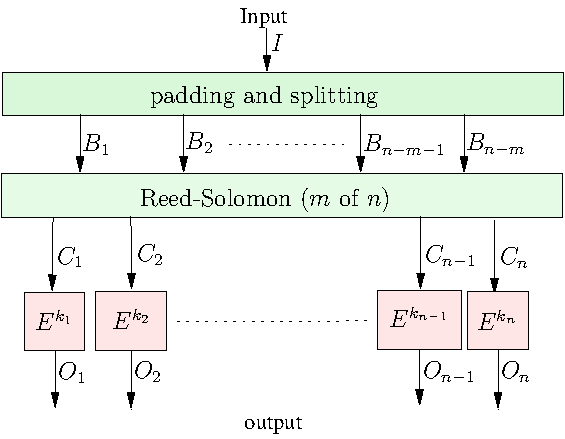
\includegraphics[width=0.8\columnwidth]{../../inc/addRedundancyOp}
	\caption{Outline of the addRedundancy operation}
	\label{fig:addRedundancyOperation}
\end{figure}
It may be subdivided into the following operations:
\begin{itemize}
	\item Pad the original message block in such a way, that all resulting blocks are a multiple of the block size of the encrypting cipher.
	\item Apply a Reed Solomon operation in a given GF space with a vanderMonde matrix.
	\item Encrypt all resulting blocks with unpadded, symmetrical encryption.
\end{itemize}

\subsection{Usage of the Protocol}

\section{Discussion of the Results}
\subsection{Static Protocol Analysis}
\subsubsection{Endpoint Operation}
\subsection{Dynamic Protocol Analysis}

\section{Conclusion}
Creating a possibly censorship resistant protocol is already hard. Analysis showed that even when a protocol is crafted with great care braking unobservability is far easier than doing it right.

\hfill gwm
 
\hfill May 8, 2019

%\subsection{Subsection Heading Here}
%Subsection text here.

% needed in second column of first page if using \IEEEpubid
%\IEEEpubidadjcol

%\subsubsection{Subsubsection Heading Here}
%Subsubsection text here.


% An example of a floating figure using the graphicx package.
% Note that \label must occur AFTER (or within) \caption.
% For figures, \caption should occur after the \includegraphics.
% Note that IEEEtran v1.7 and later has special internal code that
% is designed to preserve the operation of \label within \caption
% even when the captionsoff option is in effect. However, because
% of issues like this, it may be the safest practice to put all your
% \label just after \caption rather than within \caption{}.
%
% Reminder: the "draftcls" or "draftclsnofoot", not "draft", class
% option should be used if it is desired that the figures are to be
% displayed while in draft mode.
%
%\begin{figure}[!t]
%\centering
%\includegraphics[width=2.5in]{myfigure}
% where an .eps filename suffix will be assumed under latex, 
% and a .pdf suffix will be assumed for pdflatex; or what has been declared
% via \DeclareGraphicsExtensions.
%\caption{Simulation results for the network.}
%\label{fig_sim}
%\end{figure}

% Note that the IEEE typically puts floats only at the top, even when this
% results in a large percentage of a column being occupied by floats.
% However, the Computer Society has been known to put floats at the bottom.


% An example of a double column floating figure using two subfigures.
% (The subfig.sty package must be loaded for this to work.)
% The subfigure \label commands are set within each subfloat command,
% and the \label for the overall figure must come after \caption.
% \hfil is used as a separator to get equal spacing.
% Watch out that the combined width of all the subfigures on a 
% line do not exceed the text width or a line break will occur.
%
%\begin{figure*}[!t]
%\centering
%\subfloat[Case I]{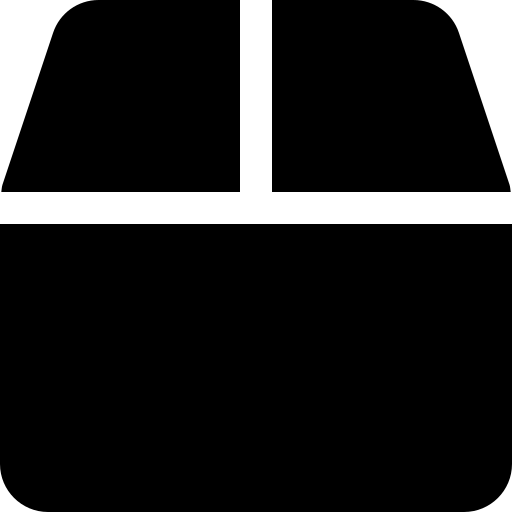
\includegraphics[width=2.5in]{box}%
%\label{fig_first_case}}
%\hfil
%\subfloat[Case II]{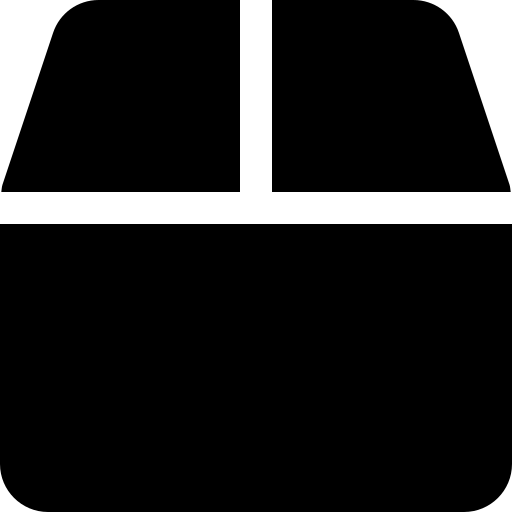
\includegraphics[width=2.5in]{box}%
%\label{fig_second_case}}
%\caption{Simulation results for the network.}
%\label{fig_sim}
%\end{figure*}
%
% Note that often IEEE papers with subfigures do not employ subfigure
% captions (using the optional argument to \subfloat[]), but instead will
% reference/describe all of them (a), (b), etc., within the main caption.
% Be aware that for subfig.sty to generate the (a), (b), etc., subfigure
% labels, the optional argument to \subfloat must be present. If a
% subcaption is not desired, just leave its contents blank,
% e.g., \subfloat[].


% An example of a floating table. Note that, for IEEE style tables, the
% \caption command should come BEFORE the table and, given that table
% captions serve much like titles, are usually capitalized except for words
% such as a, an, and, as, at, but, by, for, in, nor, of, on, or, the, to
% and up, which are usually not capitalized unless they are the first or
% last word of the caption. Table text will default to \footnotesize as
% the IEEE normally uses this smaller font for tables.
% The \label must come after \caption as always.
%
%\begin{table}[!t]
%% increase table row spacing, adjust to taste
%\renewcommand{\arraystretch}{1.3}
% if using array.sty, it might be a good idea to tweak the value of
% \extrarowheight as needed to properly center the text within the cells
%\caption{An Example of a Table}
%\label{table_example}
%\centering
%% Some packages, such as MDW tools, offer better commands for making tables
%% than the plain LaTeX2e tabular which is used here.
%\begin{tabular}{|c||c|}
%\hline
%One & Two\\
%\hline
%Three & Four\\
%\hline
%\end{tabular}
%\end{table}


% Note that the IEEE does not put floats in the very first column
% - or typically anywhere on the first page for that matter. Also,
% in-text middle ("here") positioning is typically not used, but it
% is allowed and encouraged for Computer Society conferences (but
% not Computer Society journals). Most IEEE journals/conferences use
% top floats exclusively. 
% Note that, LaTeX2e, unlike IEEE journals/conferences, places
% footnotes above bottom floats. This can be corrected via the
% \fnbelowfloat command of the stfloats package.




%\section{Conclusion}
%The conclusion goes here.





% if have a single appendix:
%\appendix[Proof of the Zonklar Equations]
% or
%\appendix  % for no appendix heading
% do not use \section anymore after \appendix, only \section*
% is possibly needed

% use appendices with more than one appendix
% then use \section to start each appendix
% you must declare a \section before using any
% \subsection or using \label (\appendices by itself
% starts a section numbered zero.)
%


\appendices
%\section{Proof of the First Zonklar Equation}
%Appendix one text goes here.

% you can choose not to have a title for an appendix
% if you want by leaving the argument blank
%\section{}
%Appendix two text goes here.


% use section* for acknowledgment
%\ifCLASSOPTIONcompsoc
%  % The Computer Society usually uses the plural form
%  \section*{Acknowledgments}
%\else
%  % regular IEEE prefers the singular form
%  \section*{Acknowledgment}
%\fi
%
%
%The authors would like to thank...


% Can use something like this to put references on a page
% by themselves when using endfloat and the captionsoff option.
\ifCLASSOPTIONcaptionsoff
  \newpage
\fi



% trigger a \newpage just before the given reference
% number - used to balance the columns on the last page
% adjust value as needed - may need to be readjusted if
% the document is modified later
%\IEEEtriggeratref{8}
% The "triggered" command can be changed if desired:
%\IEEEtriggercmd{\enlargethispage{-5in}}

% references section

% can use a bibliography generated by BibTeX as a .bbl file
% BibTeX documentation can be easily obtained at:
% http://mirror.ctan.org/biblio/bibtex/contrib/doc/
% The IEEEtran BibTeX style support page is at:
% http://www.michaelshell.org/tex/ieeetran/bibtex/
\bibliographystyle{IEEEtran}
% argument is your BibTeX string definitions and bibliography database(s)
%\bibliography{IEEEabrv,../bib/paper}
%
% <OR> manually copy in the resultant .bbl file
% set second argument of \begin to the number of references
% (used to reserve space for the reference number labels box)
%\begin{thebibliography}{1}
%
%
%\end{thebibliography}
\bibliography{../../messageVortex}

% biography section
% 
% If you have an EPS/PDF photo (graphicx package needed) extra braces are
% needed around the contents of the optional argument to biography to prevent
% the LaTeX parser from getting confused when it sees the complicated
% \includegraphics command within an optional argument. (You could create
% your own custom macro containing the \includegraphics command to make things
% simpler here.)
%\begin{IEEEbiography}[{\includegraphics[width=1in,height=1.25in,clip,keepaspectratio]{mshell}}]{Michael Shell}
% or if you just want to reserve a space for a photo:
\gdef\bioloc{../../inc/biography/}
\begin{IEEEbiography}[{\includegraphics[width=1in,height=1.25in,clip,keepaspectratio]{\bioloc/passphoto}}]{Martin Gwerder}
  \input \bioloc/biotext.inc.tex
\end{IEEEbiography}

% if you will not have a photo at all:
%\begin{IEEEbiographynophoto}{John Doe}
%Biography text here.
%\end{IEEEbiographynophoto}

% insert where needed to balance the two columns on the last page with
% biographies
%\newpage

%\begin{IEEEbiographynophoto}{Jane Doe}
%Biography text here.
%\end{IEEEbiographynophoto}

% You can push biographies down or up by placing
% a \vfill before or after them. The appropriate
% use of \vfill depends on what kind of text is
% on the last page and whether or not the columns
% are being equalized.

%\vfill

% Can be used to pull up biographies so that the bottom of the last one
% is flush with the other column.
%\enlargethispage{-5in}



% that's all folks
\end{document}


